\documentclass[conference]{IEEEtran}
\IEEEoverridecommandlockouts
\usepackage{cite}
\usepackage[hyphens,spaces,obeyspaces]{url}
\usepackage{amsmath,amssymb,amsfonts}
\usepackage{algorithmic}
\usepackage{graphicx}
\usepackage{textcomp}
\usepackage{xcolor}
\usepackage{csquotes}
\def\BibTeX{{\rm B\kern-.05em{\sc i\kern-.025em b}\kern-.08em
    T\kern-.1667em\lower.7ex\hbox{E}\kern-.125emX}}
\begin{document}

\title{A Strategy Video-Game for Collaborative Agents with a Personality and Humoristic Dialogues\\
}

\author{\IEEEauthorblockN{Jordan Mackie}
\IEEEauthorblockA{\textit{Student}}
\and
\IEEEauthorblockN{Alice Toniolo}
\IEEEauthorblockA{\textit{Supervisor}}
\and
\IEEEauthorblockN{Christopher Stone}
\IEEEauthorblockA{\textit{Supervisor}}
}

\maketitle

\begin{abstract}

	We built a system of collaborative agents with personality driven decisions and humoristic dialogues with the goal of providing entertainment and also providing a human friendly way of interpreting agent interactions in multiagent systems. The agents were designed to play chess and given goal-based personalities that would affect their decisions and how they would interact with other agents. We gathered feedback through allowing volunteers to play against our agents and asking questions covering usability and enjoyment. Finally, we present our results and discuss further work or areas of improvement that could be taken up.

\end{abstract}

\section{Introduction}

Multiagent systems are the next step to increase the level of autonomy that can be provided by technology. Agents that are able to learn, adapt, and negotiate with other agents to achieve their goals allow for complex problems to be solved or modelled without human intervention, such as monitoring and maintaining national power grids \cite{archon}. 

Often, developers and users will anthropomorphise these agents when describing their behaviour. This project aims to encourage this by implementing agents with a model of personality that affects their choice of actions, by rendering the negotiations between agents in a natural language, and by using models of humour to make the interactions between agents entertaining. 

Chess was chosen as our strategy game as multiagent implementations have been previously investigated, though not in a configuration where agents could have conflicting goals in the same team. However, our model for determining agent actions can be applied to any other strategy game or multiagent system.

\section{Context Survey}

\subsection{Multiagent Systems in Entertainment}

Many modern video games involve the user managing multiple characters to achieve some goal, such as producing in-game resources or defending against an opponent. This sort of problem lends itself easily to multiagent systems. Instead of having one artificial intelligence engine driving the actions of all the characters, developers can create agents with a limited set of actions and some concept of progress towards their goals and allow emergent behaviour to find a solution to the problem, sometimes in surprising ways. 

\cite{sandboxmas} discuss how multiagent systems can be applied to create more realistic worlds in sandbox games. By implementing the environment, objects, and non-playable characters (NPCs) as agents, developers can create a world that reacts and adapts the player, but also operates in isolation from the character to provide a realistic setting. The concept of personalities is also mentioned as a way of allowing similar NPCs to exhibit different slightly different behaviours, such as having aggressive or relaxed driving styles.

Even in games with very simple rules and logic, multiagent systems can find interesting and complex solutions. OpenAI implemented hide-and-seek using agents, where hiders avoid the line-of-sight of the seekers \cite{openaiemergent}. The game was played in a world with randomly generated walls and objects such as ramps (for climbing over walls) and blocks (for forming barricades). What made this fascinating is that the agents were not incentivised to use these objects, but after repeatedly playing and learning, both the hiders and seekers created strategies such as blocking each other in a safe area, and even removing the objects from the other team before hiding.

Knowing that multi-agent autocurricula can realise strategies not considered by humans, \cite{masboardgames} discuss how they can be applied to strategy board games such as Diplomacy and Risk. They describe a generic framework for supporting agent-based competitive bots for board games and then implement bots for the aforementioned games. Their research suggests that for games with a large number of units and a large action space, a multi-agent approach can identify effective strategies quicker than the exhaustive methods used for chess engines. 

\subsection{Multiagent System Frameworks}

Most multiagent systems have similar requirements, and so several frameworks have been developed to bootstrap their development. \cite{massurvey} provide a very thorough survey of the frameworks currently in use today and highlight various features and drawbacks in their implementation. 

The most popular is the Java Agent Development Framework (JADE) \cite{jade}. It conforms to the FIPA standard, which is a protocol for agent communication that involves defining performatives (e.g. request, inform), language name, and other message meta-data during communication. The benefit of systems that abide this standard is that they are able to interact regardless of the technology used to implement them. JADE provides other important features such as base classes for agent functionality called behaviours, a directory facilitator (DF) agent implementation to allow agents to find each other, and an Agent Management Service that manages and tracks the lifecycle of agents and allows them to move between containers (which can exist on multiple hosts). To aid during development, JADE also incldues a GUI for debugging and manually interacting with agents.

Other frameworks provide APIs that encourage certain design patterns. For example, Jason was built to support the belief-desire-intention (BDI) design model which attempts to seperate the processing of choosing a plan from the execution of the chosen plan \cite{jason}. Jason provides many of the same functionalities as JADE, but the latter was chosen due to being slightly more flexible.

\subsection{Models of Personality and Emotion}

Creating a truly immersive video game requires characters that the player can empathise with. Robots have been shown to be able to influence human behaviour as an authority figure \cite{bossrobot} and when begging not to be turned off \cite{turnoffrobot} by expressing emotions. \cite{personalitymodel} created and demonstrated a model of personality and emotion that would allow agents to react differently to the same stimulation. For example, when a agent with an 'introverted' personality is offered help, they are less likely to accept it due to the prolonged interaction it would entail. 

\cite{skyrim} also created a model that would use personality, emotion, and social relationships to determine the behaviour of NPCs in a video game. The frequency and tone of interactions between NPCs as well as the NPC and the player were accounted for when choosing facial expressions and tone of voice during conversations. Test subjects described feeling especially attached to the NPCs that utilised this model.

A useful aspect of multiagent systems is that agents can be developed in isolation but still interact (e.g. an agent that searches for cheap transport options and an agent responsible for auctioning train tickets could be developed separately with no knowledge of the logic being used by the other). \cite{hetrogenousagents} discuss how developing heterogeneous agent systems using personalities and social structures could help when dealing with third-party agents that have been constructed to lie and exhibit selfish or uncooperative behaviour.

\subsection{Collaborative Argumentation}

Knowledge is distributed in a multiagent system therefore specialist agents need to be able to alter the beliefs of others by appealing to their individual goals. \cite{argumentation} implemented a framework that achieves this based on a scheme given by \cite{reasoning}:

\begin{displayquote}
	In the current circumstance R, we should perform action A, which will result in new circumstances S, which will realise goal G, which will promote some value V.
\end{displayquote}

Specifically, they were able to create a framework for multiple parties to discuss and collaborate which could greatly affect the design of multiagent systems that utilise it. By producing an ontology which any agents involved in the discussion understand, goals and circumstances can be conveyed through the use of predicates and concepts. Conveniently, JADE already provides an API for creating ontologies.

The overhead of argumentation required in multiagent systems can be a quick filter to determine which problems it is a suitable solution for. For example, \cite{argumentationcontext} investigated how quickly agents that used collaborative argumentation to achieve global consistency in a time-constrained task (i.e. escaping a burning building) performed. Their results suggest that optimisations or different approaches to the protocol design would likely be necessary for a real-time strategy game, but it could depend on many factors such as the number of agents, the distribution of knowledge, and more.

\subsection{Natural Language Generation}

In order to make the discussions between agents more entertaining and user-friendly to observe, our project involves using natural language generation (NLG) methods to translate the messages to plain English. \cite{owlnlg} built an NLG system for a particular ontology language (W3C Ontology Language a.k.a. OWL), which is able to construct texts corresponding to objects and their properties in the ontology in English and Greek. \cite{rdfnlg} achieved similar results for one of the other Semantic Web Formalisms (specifically RDF) and were able to produce instructions for cooking recipes from a corpus of data in a far less human-friendly format. They were even able to adjust the level of technical jargon in the resulting text to accommodate for the readers familiarity with cooking. The ontology allowed for optimised searching of the parse trees but they also required a domain corpus (i.e. existing textual recipes) in order to properly train their natural language generator. Their solutions are specific to the Semantic Web project, and would not produce "conversations" like we are planning to do, but provide a good foundation for implementing this functionality.

Generic frameworks have also been created that are not based strictly on ontologies which may also be useful. For example, SimpleNLG \cite{simplenlg} is an NLG engine that allows for valid English phrases to be constructed through a very simple Java API. 

\cite{robotgame} created a robot capable of providing dialogue while playing against a human at tic-tac-toe, but used a slot-filling technique based on templates that suffered from little flexibility and left no room for personality in dialogue creation. Contrarily, systems such as Siri and Alexa are examples of successful dialogue systems that have been able to provide assistance to humans in the form of natural language conversations by avoiding the template based approaches.

These systems instead take advantage of machine learning techniques such as deep recurrent neural networks (DRNN). \cite{dialoguesystems} surveyed projects that applied these modern techniques for NLG, and concluded that in order to account for aspects such as current state of the program during the execution of conversation as our project requires, a hybrid of the machine learning and rule based approaches may be necessary. 

\subsection{Computational Humour}

Simply reading the discussion between agents would certainly not make for an entertaining game, and so adjusting the dialogue or agent behaviour is required. However, artificial humour also has benefits for everyday computing: a smartphone that is able to sympathise with the user when it is unable to connect to a weak WiFi network or cheer them up with a joke when they miss their bus is one that the user is more likely to enjoy using. 

Unfortunately, given humour is an incredibly contextual and culture driven concept, it is no surprise that computational humour is well researched yet still not 'solved'. Jason Rutter describes why using artificial intelligence for humour is particularly challenging:

\begin{displayquote}
"Humour is a very interesting way to look at artificial intelligence because at some point something has to have two meanings, which is not easy to do with a computer." \cite{jasonrutter}
\end{displayquote}

There are three main theories of humour that are used for computational humour: superiority theory (laugh about the misfortune of others), relief theory (using taboo subjects to release tension), and incongruity theory (using lexical and structural ambiguity). The last theory is currently the most popular, and was used during the development of JAPE \cite{jape}. JAPE identifies features such as homophones to produce jokes like:

\begin{displayquote}
	"What is the difference between leaves and a car? One you brush and rake, the other you rush and brake."
\end{displayquote}

However, JAPE does not allow for much user interaction, and most textual humour generation takes the form of simple puns and riddles. Our agents could instead generate situational humour by surprising the user by diverting suddenly from expected behaviour. The Suslov Model of humour accounts for the fact that we subconsciously predict expected conclusions to situations and phrases, and that contradictions in what is the most likely direction for a conversation or situation to what was previously predicted can create a humour response \cite{suslov}.

These probabilistic models currently appear more hopeful than the rule based models used by older implementations such as JAPE. Instead, \cite{humourrnn} used an existing corpus of jokes and a recurrent neural network to produce a system capable of generating jokes and even anti-jokes (jokes without an actual punchline). Our system may be able to adopt this system for generating dialogue, and a similar model for situational humour to achieve its goal.

\section{System Design}

An existing multiagent development framework was chosen instead of rolling our own in order to abstract away matters such as message delivery and agent life-cycle management. As mentioned earlier, JADE was chosen specifically due to its flexibility and its extensive coverage of the FIPA standard that could allow our agents to interact with other implementations with ease. 
With the intention of possibly serving the game over the internet once complete, the system had to be designed to allow for communication with agents from outside of the agent platform. The 'JadeGateway' API was used with a Spring Boot server and React UI to to achieve this. Figure \ref{fig:highlevelarchitecture} provides an high level overview of the technologies at each layer.

\begin{figure}[h]
	\centering
	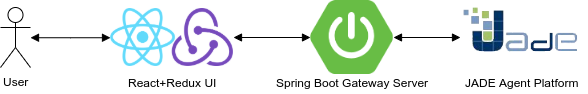
\includegraphics[width=\linewidth]{images/highlevelarchitecture}
	\caption{Technologies used at each layer.}
	\label{fig:highlevelarchitecture}
\end{figure}

\subsection{Front-End}

React \cite{reactjs} was chosen due to it being the most familiar web framework for the developer of this project, and because a component already existed for rendering chessboards \cite{chessboardjsx}. As the project grew, Redux \cite{redux} was introduced in order to help with state management of components. 
The combination of these two frameworks allowed for the use of functional components throughout the project which were easier to test due to being stateless. 

One of the challenges faced were that the abstraction of the chessboard component provided by a third-party library did not allow for atypical visual elements such as adding nametags to each piece or dialogue boxes. This then required manually implementing an overlay that would draw another chessboard grid, track positions of pieces, and draw the nametags and dialogue boxes in the correct locations.

\subsection{Agent Gateway Server}



\bibliographystyle{unsrt}
\bibliography{mybib}

\vspace{12pt}

\end{document}
